\section{Hybrid Job Placement}
\label{sec: hybrid placement}

Based on our experiments with Workloads~\Rmnum{1} and \Rmnum{2}, the ``bullying" behavior is
exhibited when the dragonfly network is configured with random placement and
(progressive) adaptive routing, and there is a large relative gap between the
communication intensity of applications running on the network.
As shown through our experimentation, contiguous placement policies give up too
much in terms of congestion and load balance, and hence are an impractical
solution. Further, running each job with a dedicated routing policy is unrealistic, 
since routing policy is part of system configuration which can not be changed
on the fly upon job submission and the policies of some jobs (adaptive)
will still interfere with others.

%Assigning preferable allocation to each job based on its communication intensity is applicable for the batch scheduler with intelligent job placement policy.


\TODO{I'll revisit this later on. As Rob mentioned, I thought we weren't
proposing a solution. (Could just need a language tweak).}
We propose a hybrid job placement policy to assign each job with preferable allocation. 
According to the hybrid placement policy, 
the less communication-intensive jobs get contiguous allocation to partially avoid network sharing with the ``bully", 
while the communication-intensive jobs get random allocation in order to share network resource with each other. 
When Workload~\Rmnum{1} is running on the dragonfly network with hybrid placement policy, 
AMG gets contiguous allocation, MultiGrid and CrystalRouter get random allocations. 


%\subsection{Network Performance Analysis}
%
%Hybrid placement is also coupled with three routing policies, minimal, adaptive and progressive adaptive, denoted respectively as HM, HA and HPA. As presented in section~\ref{sec: workload-1 network analysis} and~\ref{sec: workload-2 network analysis}, random placement outperforms contiguous placement in terms of network performance, the analysis in this section only focuses on the comparison between hybrid and random placement policies. 
%
%\begin{table}[ht]
%\begin{center}
%\caption{Average time spent on communication by all MPI ranks when Workload I is running on dragonfly network under hybrid placement and random placement policies.} 
%\label{tab: hyb-placement-wkld-commtime}
%\begin{tabular}{l c c c c c c }
%\toprule % Top horizontal line
%\toprule
%&\multicolumn{6}{c}{Placement and Routing Configurations} \\
%\cmidrule(l){2-7}
%          & HM & HA & HPA & RM & RA & RPA \\ % Column names row
%\midrule % In-table horizontal line
%Time(ms)  &273 &255 &255 &255 &265 &264  \\ % Content row 1
%%\midrule
%%Workload II &1747 &1991 &1991 &1791 &2367 &1965 \\
%\midrule % In-table horizontal line
%\bottomrule % Bottom horizontal line
%\end{tabular}
%\end{center}
%\end{table}
%
%Due to page limit, we only present the average communication time spent by Workload~\Rmnum{1} for the evaluation of the network performance.
%\footnote{The analysis about network traffic and saturated time are omitted in this section due to page limit.}
%As shown in Table~\ref{tab: hyb-placement-wkld-commtime}, 
%hybrid placement coupled with (progressive) adaptive routing (HA, HPA) can guarantee the same performance as random placement coupled with minimal routing (RM), thus the average workload communication time stays unchanged. 
%When hybrid placement coupled with minimal routing (HM) is in use, 
%the network performance declines  as indicated by the increasing average communication time. 
%The consecutive groups assigned to AMG results in the diminishing of network resource shared by MultiGrid and CrystalRouter, 
%causing unbalanced utilization over the network.  



%\subsection{Individual Application Analysis}

\begin{figure*}[t!]
    \centering
    \begin{subfigure}[t]{0.32\textwidth}
        \centering
        \includegraphics[height=1.3 in]{hyb-plcmt/mg/commtime}
        \caption{MultiGrid Communication Time}
        \label{fig:hyb-plcmt-mg-commtime}
    \end{subfigure}\hfill
    \begin{subfigure}[t]{0.32\textwidth}
        \centering
        \includegraphics[height=1.3 in]{hyb-plcmt/cr/commtime}
        \caption{CrystalRouter Communication Time}
        \label{fig:hyb-plcmt-cr-commtime}
    \end{subfigure}\hfill
    \begin{subfigure}[t]{0.32\textwidth}
        \centering
        \includegraphics[height=1.3 in]{hyb-plcmt/amg/commtime}
        \caption{AMG Communication Time}
        \label{fig:hyb-plcmt-amg-commtime}
    \end{subfigure}
   \caption{Application communication time. Workload~\Rmnum{1} is running with all placement and routing configurations.}
   \label{fig:hyb-plcmt-apps-commtime}
\end{figure*}

For the purpose of brevity, we only present the
communication time distribution of each application under all placement and routing configurations, including the hybrid placement method. These results are presented in Figure~\ref{fig:hyb-plcmt-apps-commtime}. 
As shown in Figure~\ref{fig:hyb-plcmt-mg-commtime} and~\ref{fig:hyb-plcmt-cr-commtime},
MultiGrid and CrystalRouter have similar performance with hybrid placement (HM, HA, HPA) as compared with random placement (RM, RA, RPA),
since they are still assigned with random allocations in the hybrid placement policy. 
While the performance of AMG under hybrid placement, shown in Figure~\ref{fig:hyb-plcmt-amg-commtime}, still exhibits significan communication interference on account of the other applications as opposed to the best contiguous placement policies, the effects are significantly reduced compared to a random-adaptive policy. We believe this to be a result of more AMG-specific traffic occupying a smaller set of routers/groups, both reducing the resulting probability of traffic entering them through adaptive routing and increasing the relative proportion of link utilization by AMG. Of course, this comes with the costs associated with contiguous allocation, in which AMG's traffic is less likely to load balance across multiple dragonfly groups.

\TODO{Also need to check language here. I don't think the goal is to ``solve'' the bully behavior in this work.}
The experiments with hybrid placement demonstrate that assigning each application with its preferable allocation can mitigate the negative effect of the ``bullying", in the meanwhile, 
the network can still reach the optimal performance.
Compared with random placement policy, hybrid placement can guarantee comparable network performance, by enabling network sharing between communication intensive applications .
It can also mitigate the performance degradation of less communication-intensive applications, 
by assigning them with contiguous allocation to partially avoid network sharing.
Unlike random placement indulging the ``bullying", hybrid placement can restrain it to some extent.
Hybrid placement policy is worthy of consideration for the adoption on dragonfly systems in the future.


